\section{Introduction}
\label{tW_Int}

Due to its large mass, close to the electroweak symmetry breaking scale,
the top quark is expected to play an important role in several new physics scenarios.
If the new physics scale is in the available energy range of the LHC, the existence of new
physics could be directly observed via the production of new particles. Otherwise,
new physics could affect standard model (SM) interactions indirectly,
through modifications of SM couplings or enhancements of rare SM processes.
In the latter case, it is useful to introduce a model-independent approach to parameterize and to
constrain possible deviations from SM predictions, independently of the fundamental theory of new physics.

An effective field theory (EFT) approach is followed to search for new physics in the top quark sector in the $ee$ and $\mu\mu$ final states.
In Refs.~\cite{Zhang:2010dr,Durieux:2014xla} all dimension-six
operators that contribute to the top quark pair production (\ttbar) and the single top quark production in association with a W boson (tW)
are investigated. The operators and the related effective Lagrangian, which are relevant for dilepton final states, can be written as~\cite{Grzadkowski:2010es}:
\begin{eqnarray}
\label{eq1}
O_{\phi q}^{(3)} =& (\phi^+\tau^ID_\mu\phi)(\bar{q}\gamma^\mu\tau^Iq)  ,& L_\mathit{eff}=\frac{C_{\phi q}^{(3)}}{{\sqrt 2}\Lambda^2} gv^2\bar{b}\gamma^\mu P_LtW^-_\mu+h.c.,\\
O_{tW} =& (\bar{q}\sigma^{\mu\nu}\tau^It)\tilde{\phi}W^I_{\mu\nu} ,& L_\mathit{eff}=-2\frac{C_{tW}}{\Lambda^2}v\bar{b}\sigma^{\mu\nu}P_Rt \partial_\nu W^-_\mu+h.c.,\\
O_{tG} =& (\bar{q}\sigma^{\mu\nu}\lambda^A t)\tilde{\phi}G^A_{\mu\nu} ,& L_\mathit{eff}= \frac{C_{tG}}{{\sqrt 2}\Lambda^2}v\left(\bar{t}\sigma^{\mu\nu}\lambda^A t\right) G_{\mu\nu}^A +h.c.,\\
O_{G} =& f_{ABC}G^{A\nu}_\mu G^{B\rho}_\nu G^{C\mu}_\rho ,& L_\mathit{eff}= \frac{C_{G}}{\Lambda^2} f_{ABC}G^{A\nu}_\mu G^{B\rho}_\nu G^{C\mu}_\rho + h.c.,\\
O_{u(c)G} =&  (\bar{q}\sigma^{\mu\nu}\lambda^A t)\tilde{\phi}G^A_{\mu\nu}  ,& L_\mathit{eff}= \frac{C_{u(c)G}}{{\sqrt 2}\Lambda^2}v\left(\bar{u} \left(\bar{c}\right)\sigma^{\mu\nu}\lambda^A t\right) G_{\mu\nu}^A+h.c.,
\end{eqnarray}
where C$_{\phi q}^{(3)}$, C$_{tW}$, C$_{tG}$, C$_{G}$ and C$_{u(c)G}$ stand for the dimensionless Wilson coefficients, also called effective couplings.
The variable $\Lambda$ represents the energy scale beyond which new physics becomes relevant. The detailed description of the operators is given in~Refs. \cite{Zhang:2010dr,Durieux:2014xla}.
The operators $O_{\phi q}^{(3)}$ and $O_{tW}$ modify the SM interaction between W boson, top quark, and b quark (Wtb).
The operator $O_{tG}$ is called chromomagnetic dipole moment operator of the top quark.
The triple gluon field strength operator $O_G$ represents the only genuinely gluonic CP conserving term which can appear at dimension 6 within an effective strong interaction Lagrangian \cite{Cho:1994yu}.
The operators $O_{uG}$ and $O_{cG}$ lead to flavor changing neutral current (FCNC) interactions of top quark and contribute to the tW production.
The effect of introducing the new couplings C$_{\phi q}^{(3)}$, C$_{tW}$, C$_{tG}$ and C$_{u(c)G}$ can be investigated in the tW production. The chromomagnetic dipole moment operator of the top quark affects also the \ttbar ~ production. In the case of the C$_{G}$ coupling, only the \ttbar ~production is modified.
It should be noted that the $O_{tW}$ and $O_{tG}$ operators with imaginary coefficient lead to CP-violating effects.
Representative Feynman diagrams for new physics contributions in the tW and \ttbar ~production are shown in Fig.~\ref{fig-feyn}.
In this analysis we only probe CP-even dimension six operators via top quark production.

Several searches for new physics in the top quark sector including new non-SM couplings have been performed at the Tevatron and LHC colliders.
Results can be interpreted in two ways. Most of the previous analyses followed the anomalous coupling approach in which SM interactions
are extended for possible new interactions. In this study, the EFT framework with effective couplings is used for the interpretation of the results.
Constraints obtained on anomalous couplings can be translated to effective coupling bounds~\cite{Zhang:2010dr,Abazov:2012uga}.
A variety of limits have been set on the Wtb anomalous coupling through single top quark $t$-channel production
and measurements of the W boson polarisation from top quark decay by the D0~\cite{Abazov:2012uga},
$\, \,$  ATLAS \cite{Aaboud:2017aqp,Aaboud:2016hsq} $\, \, \,$ and CMS \cite{Khachatryan:2016sib,Khachatryan:2014vma} Collaborations.
Direct limits on the top chromomagnetic dipole moment have been obtained  by the CMS Collaboration at 7 TeV using top quark pair events~\cite{CMS:2014bea}.
Searches for top quark FCNC interactions have been performed at Tevatron~\cite{Abazov:2010qk,Aaltonen:2008qr} and at LHC~\cite{Khachatryan:2016sib,Aad:2015gea}
via single top quark production and limits are set on related anomalous couplings.

\begin{figure}[t]
\centering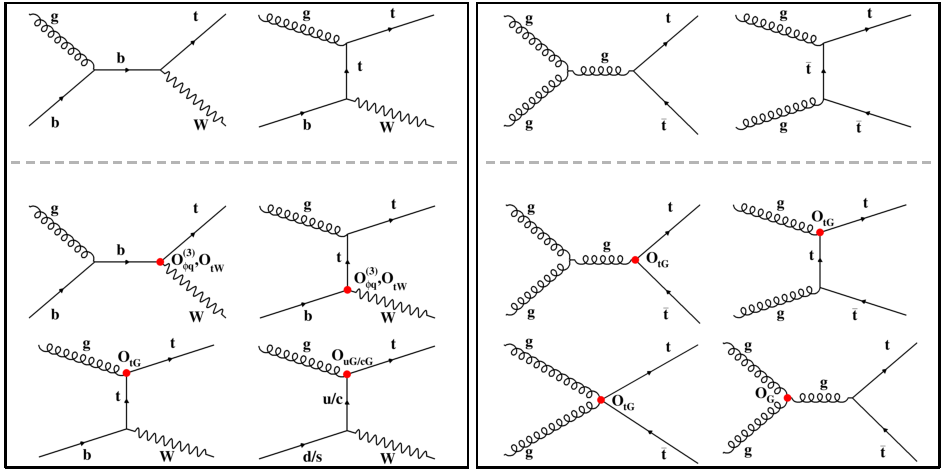
\includegraphics[width=1\textwidth]{figures/tW/fig/fey}
\caption{Representative Feynman diagrams for the tW (left panel) and \ttbar (right panel) production at leading order. The upper row gives the SM diagrams, the middle and lower rows  present diagrams corresponding to the $O_{\phi q}^{(3)}$, $O_{tW}$,$O_{tG}$, $O_{G}$ and $O_{u/cG}$ contributions.}\label{fig-feyn}
\end{figure}

In this chapter, a search for new physics in top quark production using an EFT framework is reported. Final states with two same flavor opposite-sign isolated leptons (electrons or muons) in association with jets identified as originated from the fragmentation of a b quark (``b jets'') are analysed.
%The purpose of this paper is to search for new physics in tW and \ttbar production in dilepton final state using EFT framework.
The search is sensitive to new physics contributions to the tW and \ttbar ~production, and the six effective couplings, C$_{G}$, C$_{\phi q}^{(3)}$, C$_{tW}$, C$_{tG}$, C$_{uG}$, and C$_{cG}$, are constrained independently.
Kinematic distributions of final state particles and the production rate of the tW and \ttbar ~processes are both affected by the effective couplings. For the C$_{\phi q}^{(3)}$, C$_{tW}$, C$_{tG}$, and C$_{G}$ effective couplings, the deviation from the SM prediction is dominated by the interference term between SM and new physics diagrams, which is linear with respect to the effective coupling. Therefore, kinematic distributions of final state particles vary as a function of Wilson coefficients and a small value of the effective couplings leads to distributions similar to the SM predictions.
On the other hand, the new physics terms for the C$_{uG}$ and C$_{cG}$ effective couplings do not interfere with the SM tW process, and the kinematic distributions of final state particles are determined by the new physics term independently of the SM prediction.
In this analysis, we use the rates of tW and \ttbar ~production for probing the C$_{\phi q}^{(3)}$, C$_{tW}$, C$_{tG}$, and C$_{G}$ effective couplings, while both variation in rate and kinematic distributions of final state particles are employed  for probing the C$_{uG}$ and C$_{cG}$ effective couplings.



The chapter is structured as follows. In Section \ref{tW_Samples}, a description of the data and simulated samples used in the analysis is detailed. The trigger used in this analysis is detailed in Section \ref{tW_Trigger}. The object selection and event selection are presented in Section \ref{tW_Objectselection} and \ref{tW_Eventselection}, respectively. The SM background estimation and data mc distribution are presented in sections \ref{tW_background} and Section \ref{tW_data_mc}, respectively.
Section \ref{signal} presents a description of the signal extraction procedure.
An overview of the systematic uncertainty treatment is given in Section \ref{tW_systematic}. A cross check for measuring SM tW process cross section is provided in appendix \ref{App_tW_XS}.
Finally, the constraints on the effective couplings are presented in Section \ref{tW_Results}, and a summary is given in Section \ref{sec:tW_summary}.
